\section{CREATIONAL PATTERNS}
\subsection{Singleton}

\paragraph{}
The Singleton pattern assure that the number of objects of the classes implementing this pattern are limited to one. The reason for this restriction is that, the object of this class would hold the global resource, and the creation of new object could be meaningless.

\paragraph{}
I have implemented this pattern in a lot of classes. Some of them are CityFactory, FlightFactory, CheapHotelStrategy, PoolTicketStrategy, TravelBuilder.

\paragraph{}
Below is a piece of code from class TravelBuilder, which implement Singleton

\begin{lstlisting}
private static TravelBuilder instance;

private TravelBuilder() {

}

public static TravelBuilder getInstance() {
	if (instance == null)
		instance = new TravelBuilder();
	return instance;
}
\end{lstlisting}

The constructor is set to private, so no other class can use this constructor to create new object of this class. Instead, we could call the static function \textit{getInstance} to get the only instance of TravelBuilder.

\newpage
\subsection{Abstract Factory}
The Abstract Factory pattern is used, when there are many factories of related objects. In this case, FlightFactory, CityFactory, HotelFactory are the factories of Flight, City, Hotel. 

\begin{figure}[h]
\centering
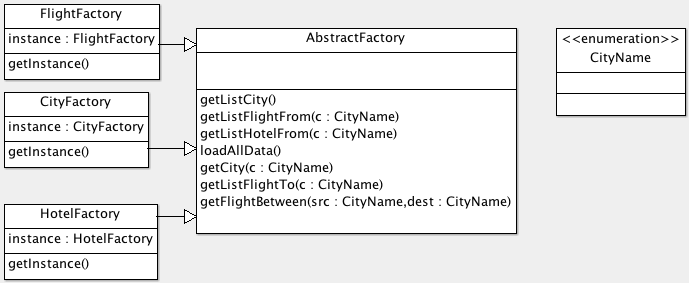
\includegraphics[width=12cm]{project/images/factory.png}
\caption{Class diagram of DataAbstractFactory}
\end{figure}

\subsection{Builder}